\documentclass[]{article}
\usepackage{graphicx}
\usepackage{indentfirst}

\usepackage{clrscode3e}
\setlength{\parindent}{0pt}

%clrs code is good!

\title{HW03 for ECE 9343}
\author{Tongda XU, N18100977}

\begin{document}

\maketitle

\section{Question 1: CLRS Problem 7.1}

\subsection{a}
This is certain concerning the $Randomized$ procedure, the probability of any index $i$ is chosen from $[0,n-1]$is:\\
$Pr(pivot = i) = \frac{1}{n}$\\
$E(X_{i}) = 1*Pr(pivot = i) + 0*Pr(pivot \neq i) = \frac{1}{n}$

\subsection{b}
It is certain that if $ith$ element is chosen as pivot, $Random-Parition$ cost $\Theta(n)$ time, and it will call $QuickSort[1, q-1], QuickSort[q+1, n]$ recursively.\\
Concerning only the first $Parition$, this would be the result:\\
$E(T(n)) = \Sigma_{i=1}^{n}Pr(pivot = i)(T(i-1) + T(n-i) + \Theta(n))\\
= \Sigma_{i=1}^{n}X_{i}(T(i-1) + T(n-i) + \Theta(n))$

\subsection{c}
Concerning $X_{i} = \frac{1}{n}\\
E(T(n)) = \Sigma_{i=1}^{n}\frac{1}{n}(T(i-1) + T(n-i) + \Theta(n))\\
= \Sigma_{i=1}^{n}\frac{1}{n}T(i-1) + \Sigma_{i=1}^{n}\frac{1}{n}T(n-i) + \Sigma_{i=1}^{n}\frac{1}{n}\Theta(n)\\
= \frac{2}{n}\Sigma_{i=1}^{n-1}T(i) + \Theta(n)$

\subsection{d}
$\Sigma_{k=2}^{n-1}klgk \\
\le lg\frac{n}{2}\Sigma_{k=2}^{\frac{n}{2}}k + lgn\Sigma_{k=\frac{n}{2}}^{n-1}k\\
= lgn\Sigma_{k=2}^{n-1}k - lg2\Sigma_{k=2}^{\frac{n}{2}}k\\
= lgn\frac{(n+1)(n-2)}{2} - \frac{(\frac{n}{2} + 2)(\frac{n}{2}-1)}{2}\\
\le lgn\frac{n^2}{2} - \frac{n^2}{8}$\\
by Calculus, we have:\\
$(\frac{1}{2}x^2lgx - \frac{1}{4}x^2)|_{1}^{n-1} \le E(T(n)) \le (\frac{1}{2}x^2lgx - \frac{1}{4}x^2)|_{2}^{n}$

\subsection{e}
Proof of $E(T(n)) = O(nlgn)$:\\
Assume that $\forall k \in [1, n-1], \exists c, E(T(k)) \le cklgk - \Theta(k)$\\
For $k = n, E(T(n)) \le \frac{n}{2}c(lgn\frac{n^2}{2} - \frac{n^2}{4} - \Theta (n^2)) + \Theta(n) \le cnlgn - \Theta(n) $\\
Proof of $E(T(n)) =\Omega(nlgn)$:\\
Assume that $\forall k \in [1, n-1], \exists c, E(T(k)) \ge cklgk + \Theta(k)$\\
For $k = n, E(T(n)) \ge \frac{n}{2}c(lgn\frac{(n-1)^2}{2} - \frac{(n-1)^2}{4} + \Theta(n^2)) + \Theta(n) \ge cnlgn + \Theta(n)$\\
$\rightarrow E(T(n)) = \Theta(nlgn)$

\section{Question 2: CLRS Problem 7.5}

\subsubsection{a}
From counting Theorem, it could be noticed that:\\
$p_{i} = \frac{(i-1)(n-i)}{C_{n}^{3}} = \frac{6(i-1)(n-i)}{n(n-1)(n-2)}$

\subsubsection{b}
$Pr(i = medium) (normal) = \frac{1}{n}\\
Pr(i = medium) (3part) = \frac{6(\frac{1}{2}n-1)(n-\frac{1}{2}n)}{n(n-1)(n-2)} = \frac{3}{2}\frac{1}{n}\\
Pr(3part) - Pr(normal) = \frac{1}{2}\frac{1}{n}$

\subsubsection{c}
Consider $f_{diff}= {\int }_{\frac{n}{3}}^{\frac{2}{3}n} (\frac{6(i-1)(n-i)}{n(n-1)(n-2)} - \frac{1}{n})di\\
= \frac{(-2i^3 + 3(n+1)i^2 - 6ni - (n-1)(n-2)i)|_{i = \frac{1}{3}n}^{i = \frac{2}{3}n}}{n(n-1)(n-2)}\\
{lim}_{n\to \infty} f_{diff} = \frac{4}{27}$

\subsubsection{d}
Consider we are so lucky that each partition we choose the median:\\
In the Iteration tree, we have:\\
$ T(n)=\left\{
\begin{array}{lcl}
c       &      & {n = 1}\\
2T(\frac{1}{2}n) + n     &      & {n > 1}\\
\end{array} \right. $\\
The $\Omega(nlgn)$ is kept even in best case.

\section{Question 3: Illustrate COUNTING-SORT}
See Figure~\ref{fig:3}

\begin{figure}
	\centering
	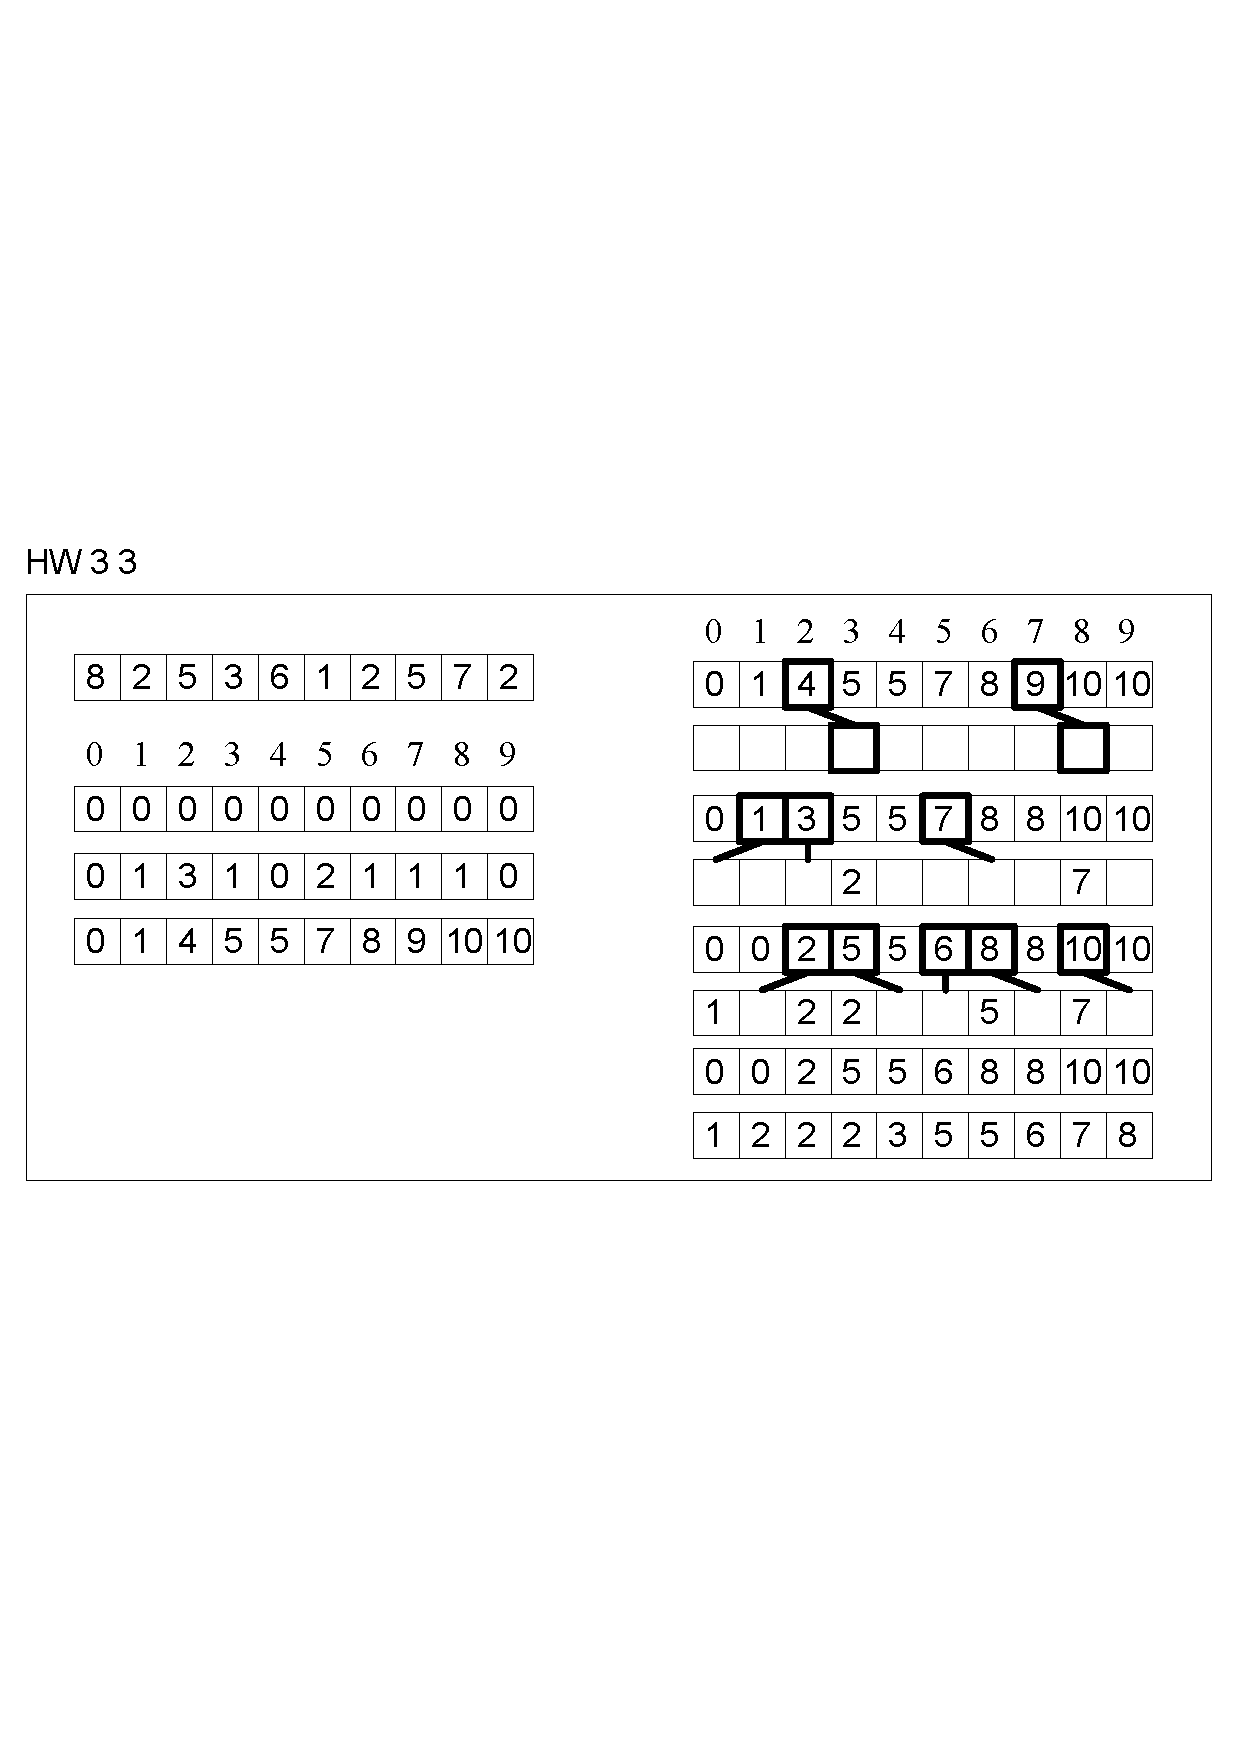
\includegraphics[width=\linewidth]{3_count}
	\caption{Question 3}
	\label{fig:3}
\end{figure}

\section{Question 4: CLRS Exercise 8.2-4}
Consider a trim version of counting sort, build the $C$ map up and query directly:\\
\begin{codebox}
	\Procname{$\proc{Counting-sort-trim($A, k$)}$}
	\li $C []$
	\li \For $i \gets 0$ \To $k$
	\li		\Do $C[i] = 0$
	\End
	\li \For $j \gets 1$ \To $A.length$
	\li		\Do $C[A[j]]++$
	\End
	\li \For $m \gets 1$ \To $k$
	\li		\Do $C[m] += C[m-1]$
	\End
	\li \Return $C[m]$
\end{codebox}

\begin{codebox}
	\Procname{$\proc{Direct-Quert($A, k, a, b$)}$}
	\li $C = \proc{Counting-sort-trim($A, k$)}$
	\li \If $a < 1$
	\li \Then \Return $C[b]$
	\li \Else \Return $C[b] - C[a-1]$
\end{codebox}

\section{Question 5: CLRS Exercise 8.3-4}
First, with $O(n)$ time: convert n numbers $k_{10}$ into $k_{n}$ which has 3 digits.\\
Second, with $O(d(n+n))$ time ($Lemma8.3$): Radix sort n 3-digit numbers with each digits take up to n possible values.

\begin{codebox}
	\Procname{$\proc{digitsConvert($X$)}$}
	\li $result []$
	\li \For $i \gets 2$ \Downto $0$
	\li		\Do $result[i] = X/n^i$
	\li			$X = X \bmod{n^i}$
	\End
	\li \Return $result$
\end{codebox}

\begin{codebox}
	\Procname{$\proc{sort($A,x$)}$}
	\li $result []$
	\li \For each $S$ in $A$
	\li		\Do $S =\proc{digitsConvert($S$)}$
	\End
	\li \proc{radix-sort($A,x$)}
\end{codebox}

\section{Question 6: CLRS Problem 9.1}

\subsection{a}

Sorting: $\proc{Merge-sort($A$)}$ in worst case $O(nlgn)$\\
Query: $\proc{call-by-rank($A,k$)}$ i times in worst case $O(i)$, here we assume manipulating $O(n)$ space cost $O(n)$ time.

\subsection{b}

Building: $\proc{build-map-heap($A$)}$ in worst case $O(n)$\\
Query: calling $\proc{Extra-max($A,k$)}$ i times in worst case $O(ilgn)$

\subsection{c}

Selecting: $\proc{select($A, i$)}$ in worst case $O(n)$\\
Sorting:  $\proc{Merge-sort($A^{'}$)}$ in worst case $O(ilgi)$

\section{Question 7: CLRS Problem 11.2}

\subsection{a}

Consider for a ball i fall into a specific bucket $Pr(i) = \frac{1}{n}$\\
Then consider Binomial Distribution, $Pr(k) = C_{n}^{k}Pr(i)^{k}(1-Pr(i))^{n-k}$

\subsection{b}

Consider random picking a slot, the probability of that slot is maximum is $Pr_{max} = \frac{1}{n}$, and it contains k elements $Q_{k}$. for conditional probability, we have:\\
$P_{k} = Pr_{i=k|max} = \frac{Pr(i=k \cap max)}{Pr_{max}} \le \frac{Pr(i=k)}{Pr_{max}} = nQ_{k}$

\subsection{c}

Proof:\\
$Q_k = (\frac{1}{n})^k(\frac{n-1}{n})^{n-k}C_{n}^{k} \\
= \frac{(n-1)^{n-k}}{n^n} \frac{\Pi_{0}^{k-1}n-k}{k!} \\
\le \frac{n^n}{n^n} \frac{1}{k!}\\
= \frac{e^k}{k^k} \frac{1}{k^{\frac{1}{2}} (1+\Theta(\frac{1}{n}))}\\
\le \frac{e^k}{k^k}$

\subsection{d}

Proof for $Q_{k_{0}}$: \\
$Q_{k_{0}} = \frac{e^{(\frac{clgn}{lglgn})}}{(\frac{clgn}{lglgn}) ^ {\frac{clgn}{lglgn}}}\\
= \frac{n^{\frac{clg\frac{e}{c}}{lglgn}}}{\frac{n^c}{n^{\frac{clglglgn}{lglgn}}}} = n^{\frac{clg\frac{e}{c} + clglglgn}{lglgn} - c}$\\
It would not take effort to notice that since ${lim}_{n\to \infty}\frac{clg\frac{e}{c} + clglglgn}{lglgn} =0\\
\forall c > 3+\epsilon, Q_{k_{0}} = O(\frac{1}{n^3}) $\\
And $P_{k} \le nQ_{k} \rightarrow P_{k} = O(\frac{1}{n^2})$

\subsection{e}

$E(M) = \Sigma_{M = 1}^{n} M Pr(M) < nPr(M>\frac{clgn}{lglgn}) + \frac{clgn}{lglgn}Pr(M \le \frac{clgn}{lglgn})\\$
A stronger conclusion to note: \\
$E(M) = \Sigma_{M = 1}^{n} M Pr(M) < MPr(M>\frac{clgn}{lglgn}) + \frac{clgn}{lglgn}Pr(M \le \frac{clgn}{lglgn})\\
\le \int_{\frac{clgn}{lglgn}}^{\infty}\frac{1}{n}dn + 1*\frac{clgn}{lglgn} \\
= lg (\frac{clgn}{lglgn}) + \frac{clgn}{lglgn}\\ = O(\frac{clgn}{lglgn})$

\end{document}
